\section*{1. Структура \texttt{\_IO\_FILE}}

\begin{lstinputlisting}[
	caption={Структура \texttt{\_IO\_FILE}},
	style={c},
	]{../src/struct_io_file.c}
\end{lstinputlisting}

\clearpage

\section*{2. Первая программа}

\begin{figure}[h!btp]
	\centering
	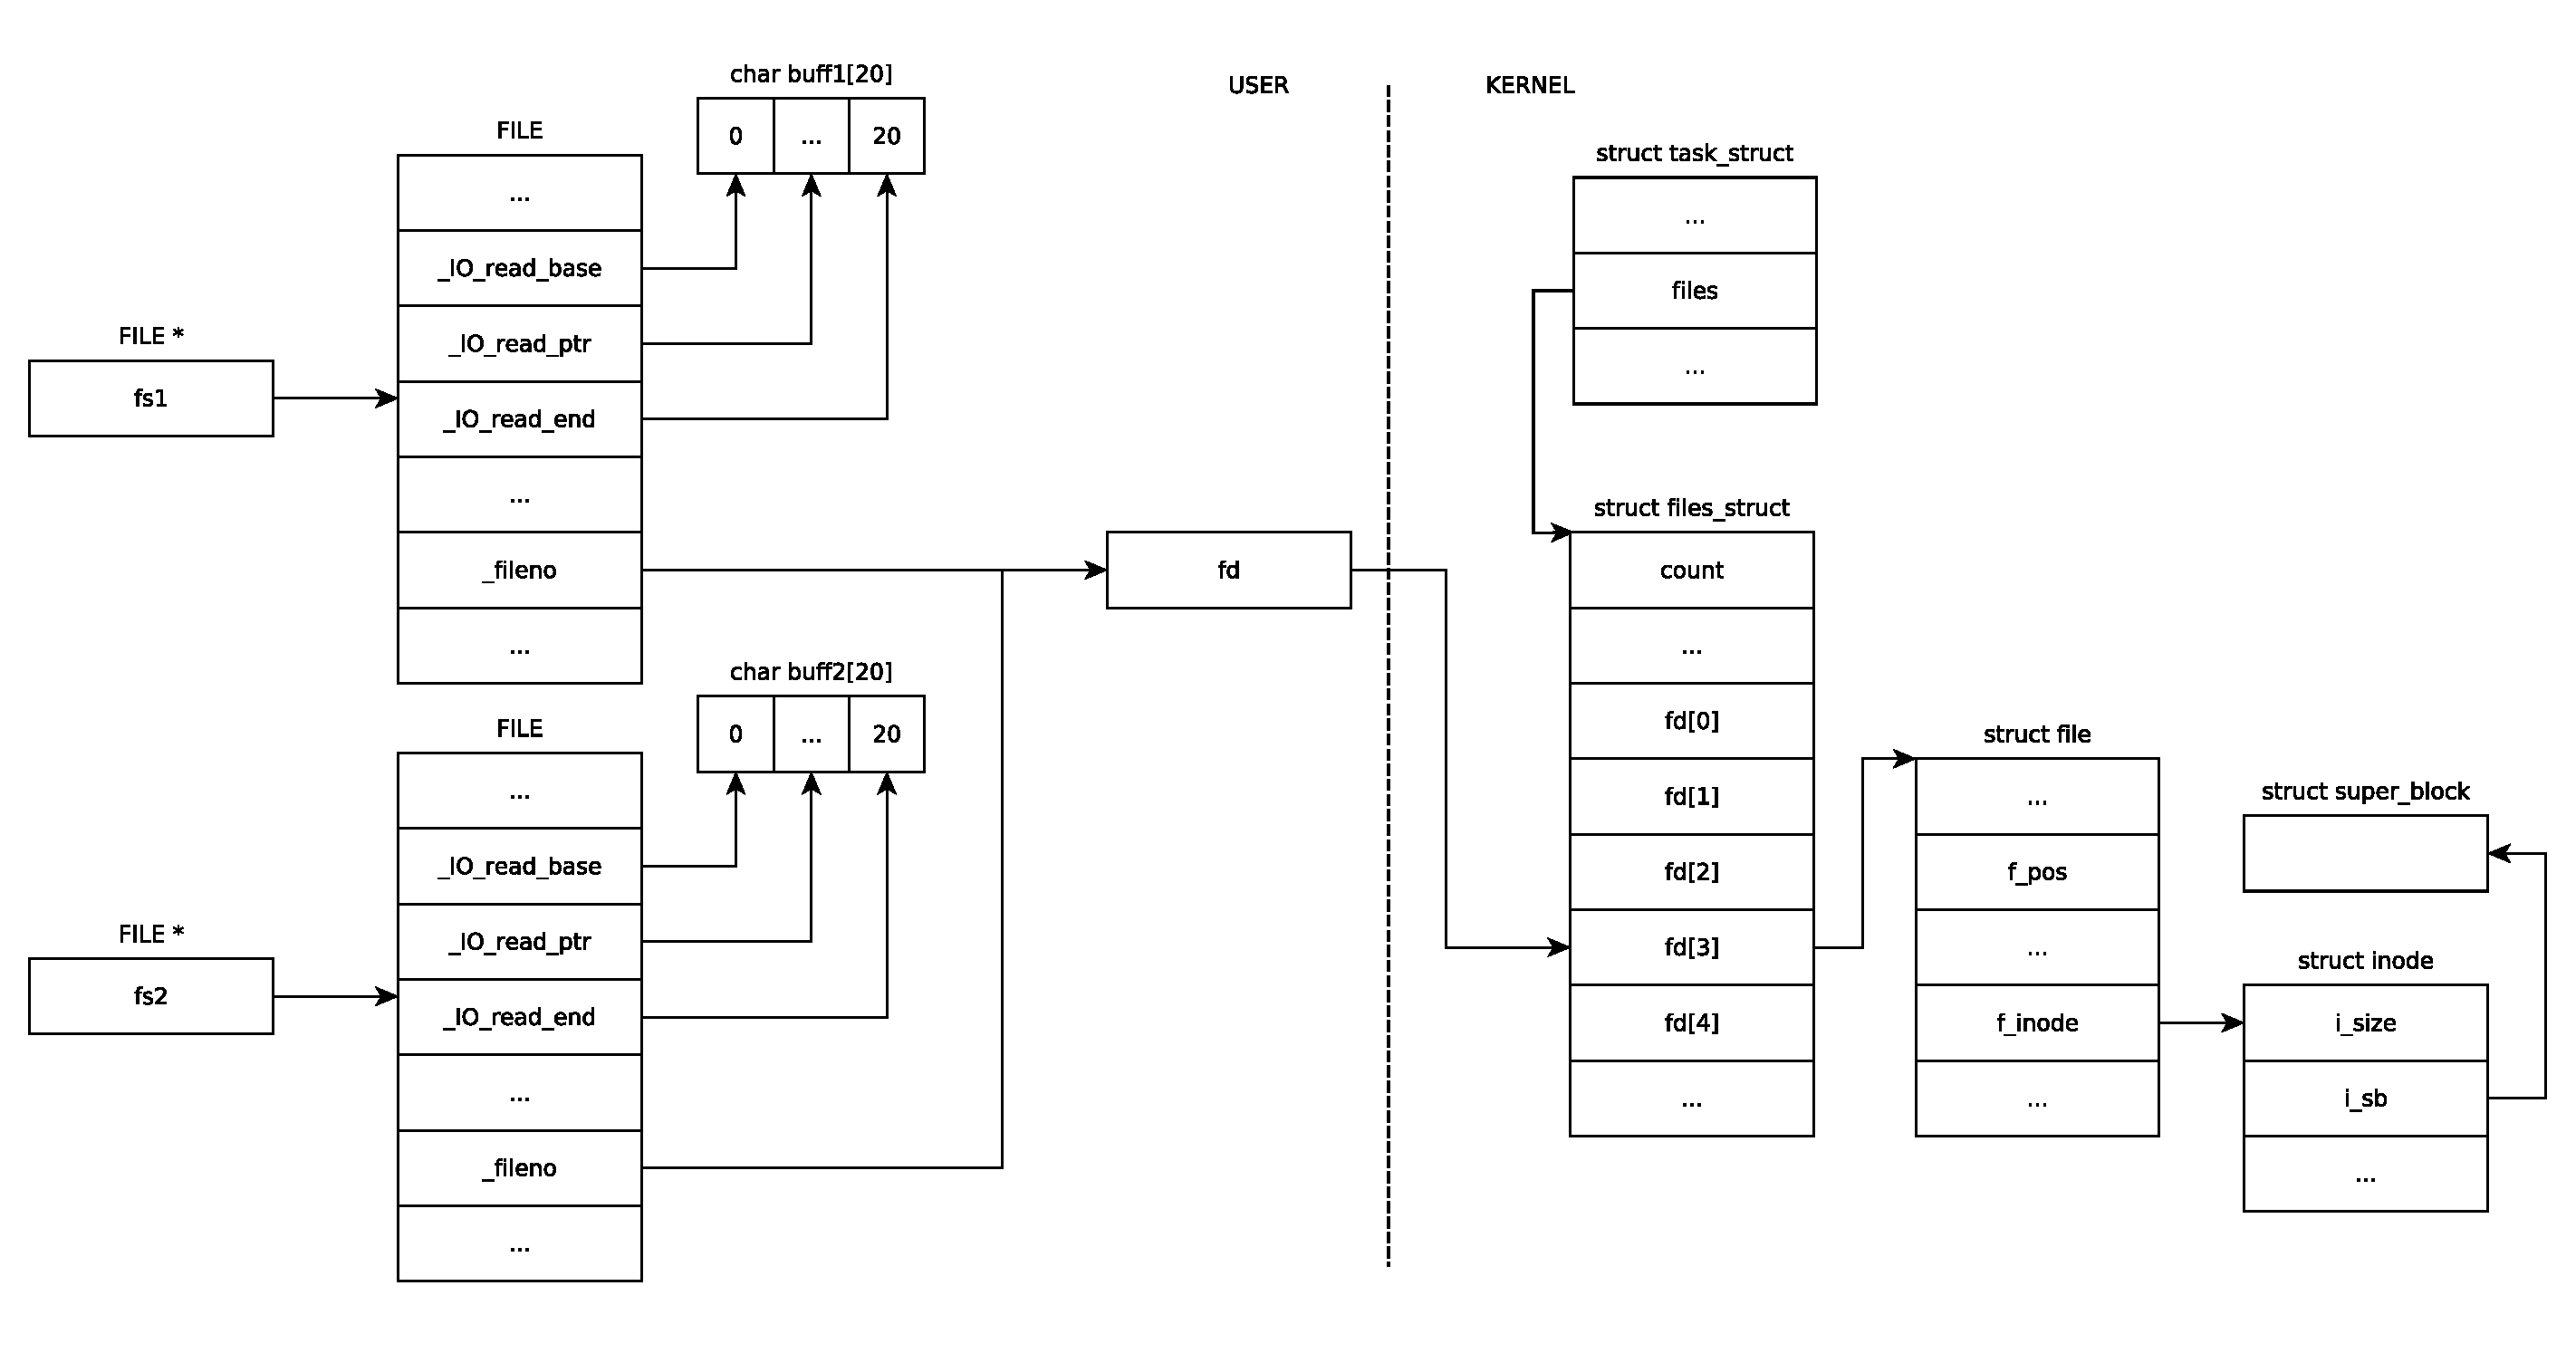
\includegraphics[width=490pt]{inc/scheme1.pdf}
	\caption{Используемые структуры}
	\label{fig:scheme1}	
\end{figure}

\begin{itemize}
	\item Функция \texttt{open()} создает новый файловый дескриптор \texttt{fd} файла (открытого только на чтение) ''\texttt{alphabet.txt}'' запись в системной таблице открытых файлов. Эта запись регистрирует смещение в файле и флаги состояния файла

	\item Функция \texttt{fdopen()} создаёт указатели на структуру \texttt{FILE}. Поле \texttt{\_fileno} содержит дескриптор, который вернула функция \texttt{fopen()}

	\item Функция \texttt{setvbuf()} явно задает размер буффера в 20 байт и меняет тип буферизации	(для \texttt{fs1} и \texttt{fs2}) на полную

	\item При первом вызове функции \texttt{fscanf()} в цикле (для \texttt{fs1}), \texttt{buff1} будет заполнен полностью -- первыми 20 символами (буквами алфавита). \texttt{f\_pos} в структуре \texttt{struct\_file} открытого файла увеличится на 20

	\item При втором вызове \texttt{fscanf()} в цикле (для \texttt{fs2}) буффер \texttt{buff2} будет заполнен оставшимися 6 символами (начиная с \texttt{f\_pos})

	\item В цикле поочерёдно выводятся символы из \texttt{buff1} и \texttt{buff2}
\end{itemize}

\clearpage

\begin{lstinputlisting}[
	caption={Исходный код первой программы},
	style={c},
	]{../src/1.c}
\end{lstinputlisting}

\begin{figure}[h!btp]
	\centering
	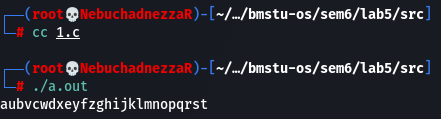
\includegraphics[width=400pt]{inc/1.png}
	\caption{Результат работы первой программы}
	\label{fig:res1}	
\end{figure}

\clearpage

\begin{lstinputlisting}[
	caption={Исходный код первой программы (многопоточная)},
	style={c},
	]{../src/1m.c}
\end{lstinputlisting}

\begin{figure}[h!btp]
	\centering
	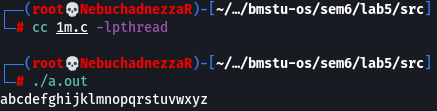
\includegraphics[width=400pt]{inc/1m.png}
	\caption{Результат работы первой программы (многопоточная)}
	\label{fig:res1m}	
\end{figure}

\clearpage

\section*{3. Вторая программа}

\begin{figure}[h!btp]
	\centering
	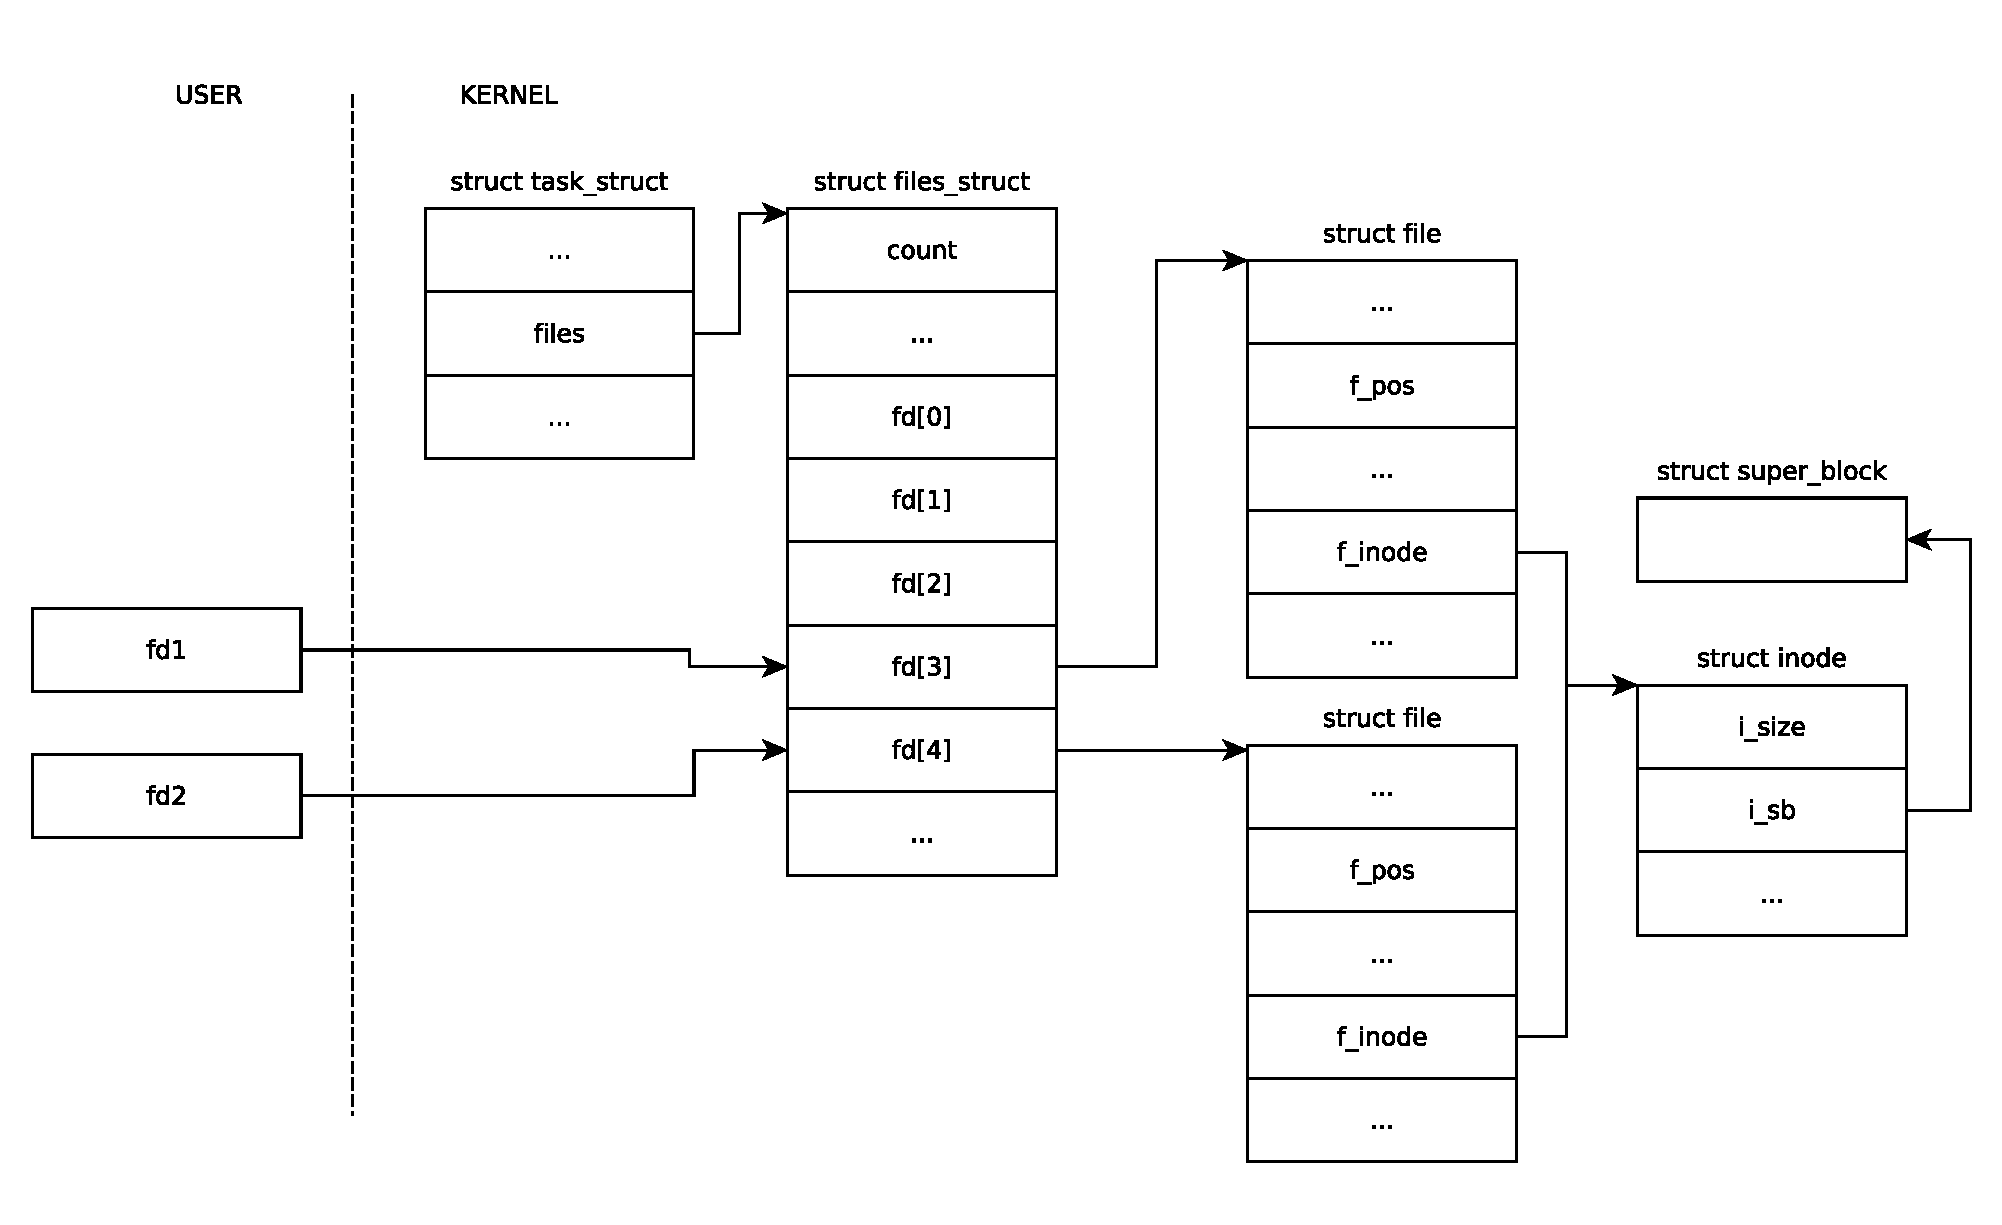
\includegraphics[width=490pt]{inc/scheme2.pdf}
	\caption{Используемые структуры}
	\label{fig:scheme2}	
\end{figure}

\begin{itemize}
	\item Функция \texttt{open()} создаёт файловые дескрипторы, два раза для одного и того же файла, поэтому в программе существует две различные \texttt{struct file}, но ссылающиеся на один	и тот же \texttt{struct inode}

	\item Из-за того что структуры разные, посимвольная печать просто дважды выведет содержимое файла в формате <<\texttt{aabbcc...}>> (в случае однопоточной реализации);

	\item В случае многопоточной реализации, вывод второго потока начнётся позже (нужно время, для создание этого потока) и символы перемешаются, что видно на рисунке \ref{fig:res2m}
\end{itemize}

\clearpage

\begin{lstinputlisting}[
	caption={Исходный код второй программы},
	style={c},
	]{../src/2.c}
\end{lstinputlisting}

\begin{figure}[h!btp]
	\centering
	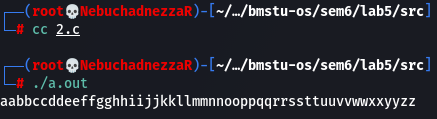
\includegraphics[width=400pt]{inc/2.png}
	\caption{Результат работы второй программы}
	\label{fig:res2}	
\end{figure}

\clearpage

\begin{lstinputlisting}[
	caption={Исходный код второй программы (многопоточная)},
	style={c},
	]{../src/2m.c}
\end{lstinputlisting}

\begin{figure}[h!btp]
	\centering
	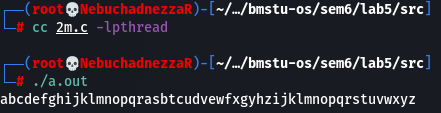
\includegraphics[width=400pt]{inc/2m.png}
	\caption{Результат работы второй программы (многопоточная)}
	\label{fig:res2m}	
\end{figure}

\clearpage

\section*{3. Третья программа}

\begin{figure}[h!btp]
	\centering
	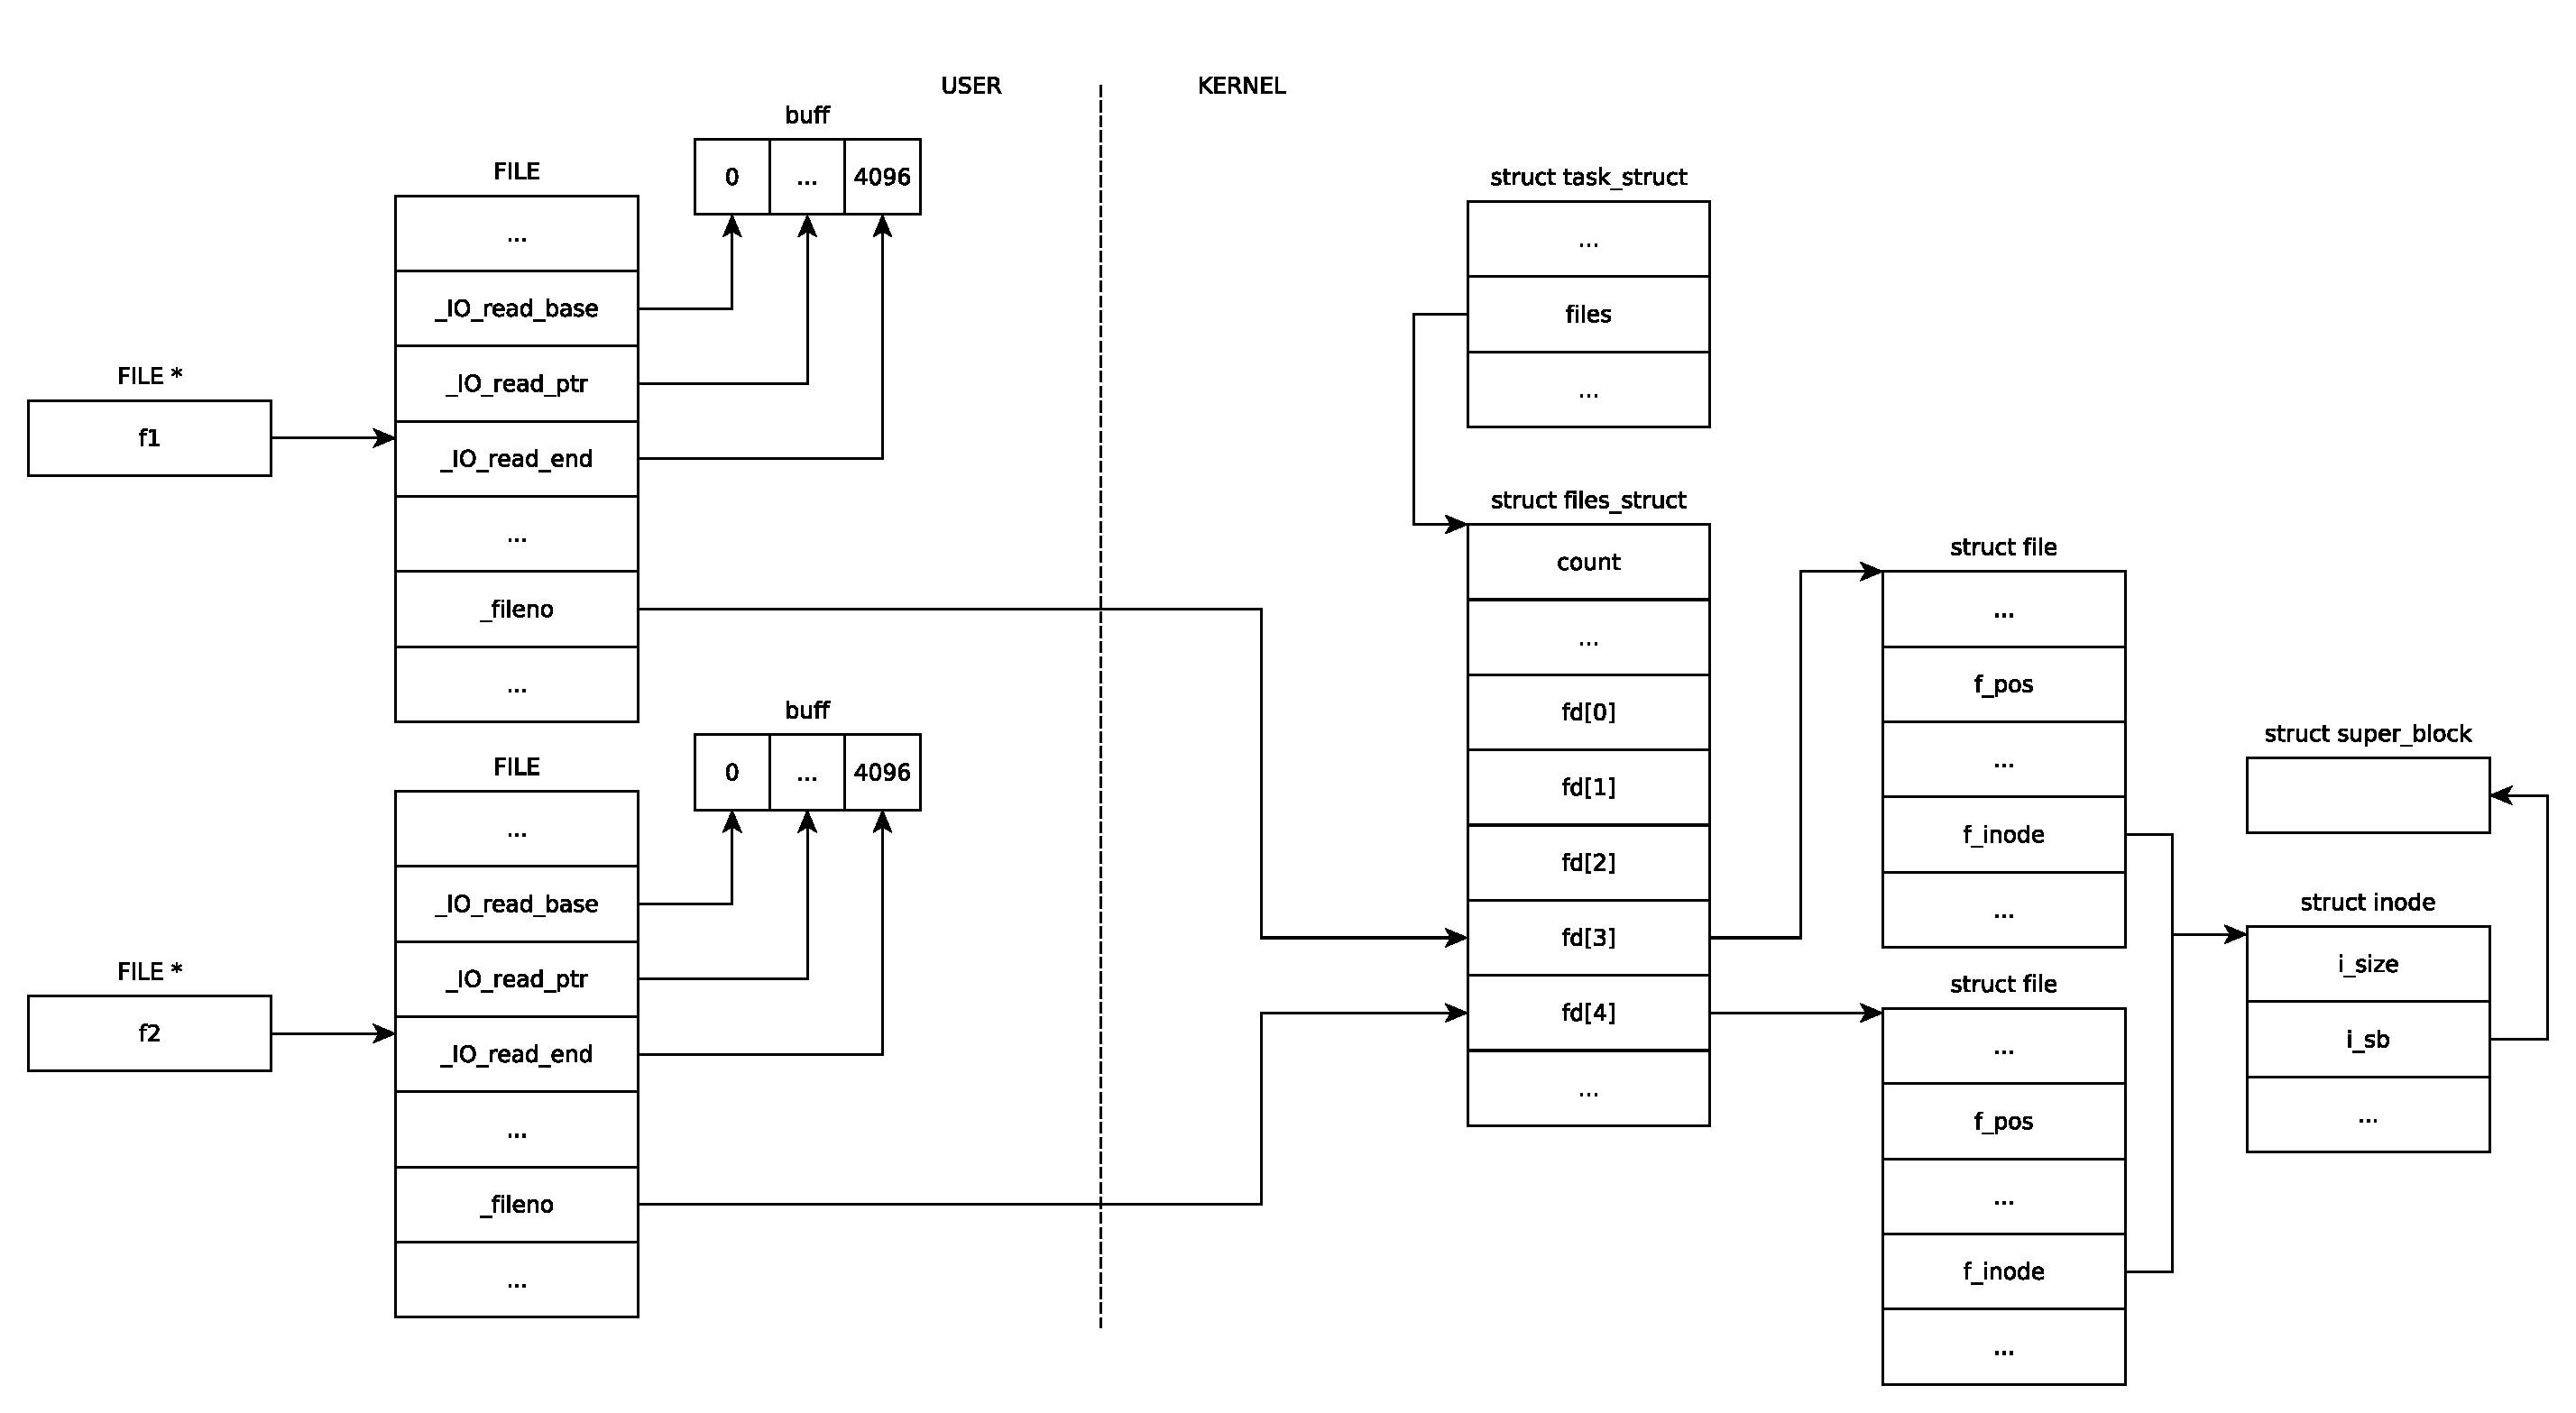
\includegraphics[width=470pt]{inc/scheme3.pdf}
	\caption{Используемые структуры}
	\label{fig:scheme3}	
\end{figure}

\begin{itemize}
	\item Файл открывается на запись два раза, с помощью функции \texttt{fopen()}

	\item Функция \texttt{fprintf()} предоставляет буферизованный вывод - буфер создаётся без нашего вмешательства

	\item Изначально информация пишется в буфер, а из буфера в файл если произошло одно из
	событий:
	\begin{enumerate}
		\item буффер полон
		\item вызвана функция \texttt{fclose()}
		\item вызвана функция \texttt{fflush()}
	\end{enumerate}

	\item В случае нашей программы, информация в файл запишется в результате вызова функция \texttt{fclose()}

	\item Из-за того \texttt{f\_pos} независимы для каждого дескриптора файла, запись в файл будет производится с самого начала
\end{itemize}

\clearpage

\begin{lstinputlisting}[
	caption={Исходный код Третьей программы},
	style={c},
	]{../src/3.c}
\end{lstinputlisting}

\begin{figure}[h!btp]
	\centering
	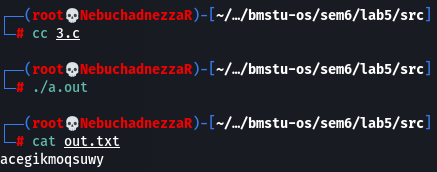
\includegraphics[width=400pt]{inc/3.png}
	\caption{Результат работы третьей программы}
	\label{fig:res3}	
\end{figure}

\clearpage

\begin{lstinputlisting}[
	caption={Исходный код третьей программы (многопоточная)},
	style={c},
	]{../src/3m.c}
\end{lstinputlisting}

\begin{figure}[h!btp]
	\centering
	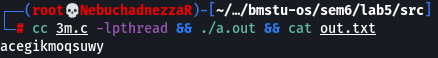
\includegraphics[width=400pt]{inc/3m.png}
	\caption{Результат работы третьей программы (многопоточная)}
	\label{fig:res3m}	
\end{figure}